\chapter{Introduction}

As researchers first started to build technology to help us communicate with other people at a distance, a consensus on what the goal should be quickly arose: computer mediated communication systems should focus on recreating the experience of being face-to-face with another person. The best system, in this model, is one that seems to disappear in the same way that the best window makes us feel like there is nothing between us and what's on the other side of the glass. Since the early 1970s, it has seemed like we have always been on the verge of a utopian environment where distance disappears and we interact as richly with friends, family, and colleagues around the world as we do with someone sitting in the same room. \citep{Egido:1988vq} And yet, like the paperless office \citep{Sellen:2001uk}, this future has failed to materialize. We can interpret this in two ways: either our tools have failed to deliver on the promise of a ``being there'' level experience or we have been aiming for the wrong target. As with \citet{Hollan:1992tz}, I will argue that the latter case is true. The persistence of a preference for face-to-face communication represents a failure on the part of designers and researchers to recognize both the subtle qualities of face-to-face communication and the potential of computer-mediated-communication tools to complement existing interaction contexts.

% might also be able to deploy a ref to Nilles, J., 1988. Traffic reduction by telecommuting: A status review and selected bibliography. Transportation Research Part A: General. Available at: http://linkinghub.elsevier.com/retrieve/pii/0191260788900088.


Core to the argument that computer-mediated-communication should simply recreate face-to-face interactions as transparently as possible is the notion that face-to-face interaction is the best we can hope for. Depending on your perspective, it may seem either heretical or obvious that we might prefer non-face-to-face interaction in certain situations. We can look to research on media selection preferences to convince ourselves that this is true.

Since computer-mediated-communication became technically viable, there has been broad interest in understanding the relative properties of speech, video, and text, as well more esoteric (and largely ignored) modalities like real-time handwriting transmission. \citep{Williams:1977p682} This stream of work can be traced back to \citet{Ochsman:1974vu}, who studied pairs of students coordinating on concrete tasks like scheduling, wayfinding, and physical part identification using different sorts of communication tools. This early work focused on measuring which channels were most effective for tasks, and primarily recommended that adding voice was the biggest improvement in performance. This type of work has continued, with researchers expanding their view beyond task performance to trust formation \citep{Bos:2002p256}\citep{Toma:2010p347} and deception \citep{Hancock:2004p314}.

% also cite the chapanis sci amer article? it's better and a little more broad

Outside of lab contexts, we are not assigned a specific tool for a specific task. Instead, we make nuanced and highly contextual choices about what sorts of tools to use in different communication situations. If we accepted the idea that ``being there'' was a primary motivation, we would expect to see people prioritizing tools that were the most like ``being there'' among the available options. This spectrum is also sometimes characterized as ``media richness'' per \citet{Daft:1986p1548}, in which the most rich media are those that are most like being face-to-face. Instead, researchers have found repeatedly that in non-lab situations, people frequently choose less rich media over more rich options. \citep{Scholl:2006p210} If richness alone does not predict people's real-life communication media selection decisions, it suggests that other features of a communication medium might also be relevant. 

% there are many other takedowns of media richness theory. Could expand those here.
% try to find some more people who find what scholl finds. I know there's lots but I don't have a handy list right now. 

These features might include:

\begin{itemize}
\item Archivability
\item Mobility
\item Revisability
\item Emotional Content
\item Synchronicity
\item Interruptability
\end{itemize}

% Going to need to be more rigorous about this list at some point and find some references that support it and provide a bit more text about each item.

Since in many contexts people choose non ``being there'' interfaces because of some of these factors, we can safely conclude that designing experiences that seek to be better than ``being there'' will likely take advantage of these sorts of design elements.


% also link to facetime?
The continued focus on ``being there'' designs by much of the communication industry, Cisco's Telepresence systems \ref{fig:cisco-telepresence} and Apple's Facetime \ref{fig:facetime} being major examples reveals a blindness to the potential benefits of mediated communication systems. Furthermore, a focus on this approach hides the many challenges of face-to-face interaction. While in one-on-one situations and very small groups it may be difficult to provide a better experience than face-to-face, I see a wide variety of challenges in interacting with groups that contain more than ten people.  A closer inspection of face-to-face interaction reveals a number of potential ways it might be improved:


\begin{itemize}
\item Not all people are equally capable of convincing performances in face-to-face interaction. This can be the result of a variety of factors, including (but not limited to) a lack of confidence in contributing in a specific context, a lack of skill with language, or the impact of a power imbalance in the situation. Many of these can be mitigated in mediated contexts\citep{Siegel:1986ve}, although mediated contexts have their own distinct performance challenges.
\item Simultaneous contribution in face-to-face situations are often viewed as impolite and are generally normatively discouraged. Particularly in large groups, this represents a pressure against contribution and requires a certain amount of overhead to negotiate turn-taking gracefully.
\item Participation in face-to-face contexts usually discloses significant information about someone's identity, while in mediated contexts there are a variety of approaches to limiting disclosure of identity information while still being an active participant.
\item Face-to-face interactions are traditionally ephemeral and difficult to record; mediated interactions are usually quite easy to record. 
\end{itemize}


% I want to be able to cite the commercials, but it's a nightmare finding any information about them that might make them citable like where they appeared, when they appeared, who directed them, etc.


\begin{marginfigure}
	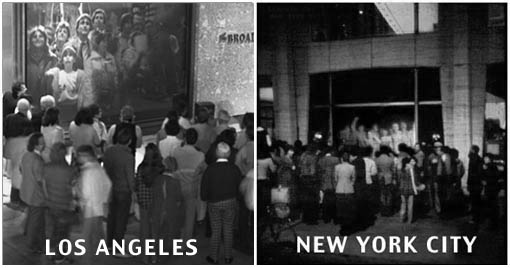
\includegraphics{figures/hole_in_space.jpg}
	\caption{Photos of the Hole in Space exhibit sites in Los Angeles and New York City.}
	\label{fig:hole-in-space}
\end{marginfigure}

\begin{marginfigure}
	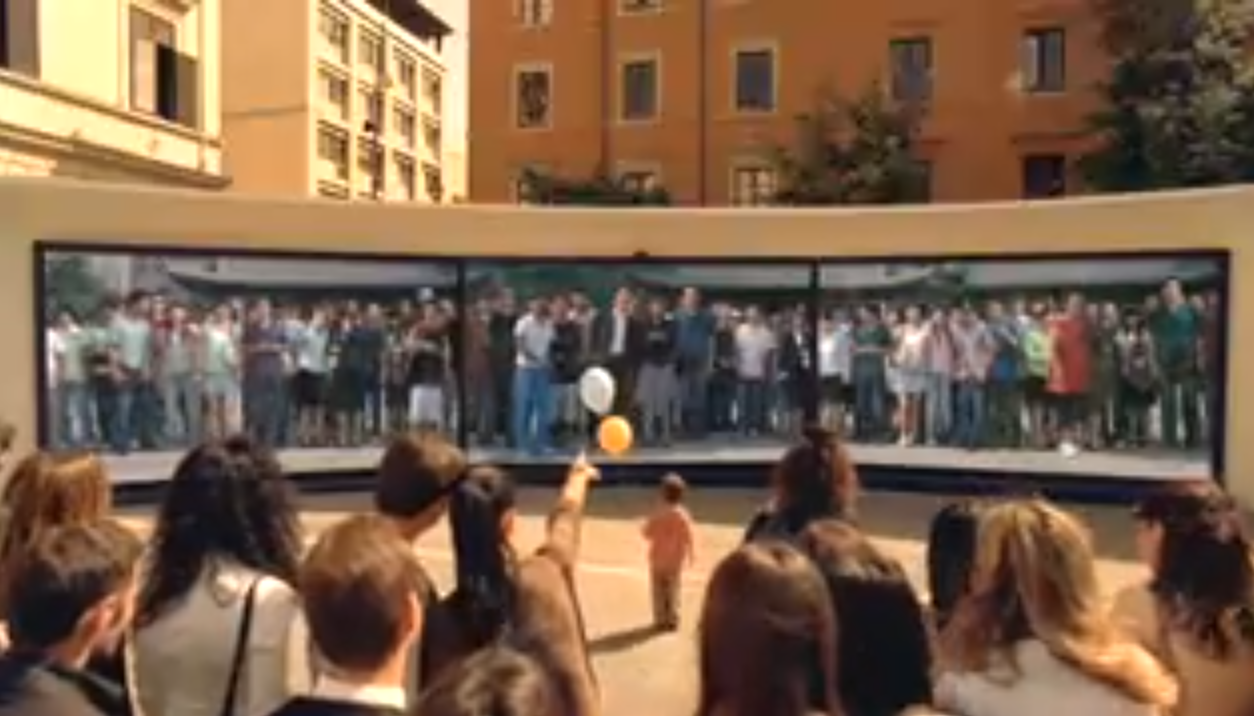
\includegraphics{figures/cisco-telepresence.png}
	\caption{Still from a Cisco Telepresence advertisement, centered on connecting an Italian piazza with a Chinese square with a seamless window.}
	\label{fig:cisco-telepresence}
\end{marginfigure}

Despite these challenges, there's still an undeniable magic to the pursuit of recreating face-to-face communication at a distance. This magic is most poetically captured in the famous ``Hole in Space'' \citep{HoleinSpace:1980vn} piece, visually and audibly connecting a storefront in Los Angeles and New York in a way that seemed to make distance disappear. This vision is not simply aspirational, either. Tools to communicate with physically distant people either with audio alone or with an added video connection play a role in the daily lives of millions of people. This desire to experience ``being there'' with someone else is powerful and compelling. 


\begin{marginfigure}
	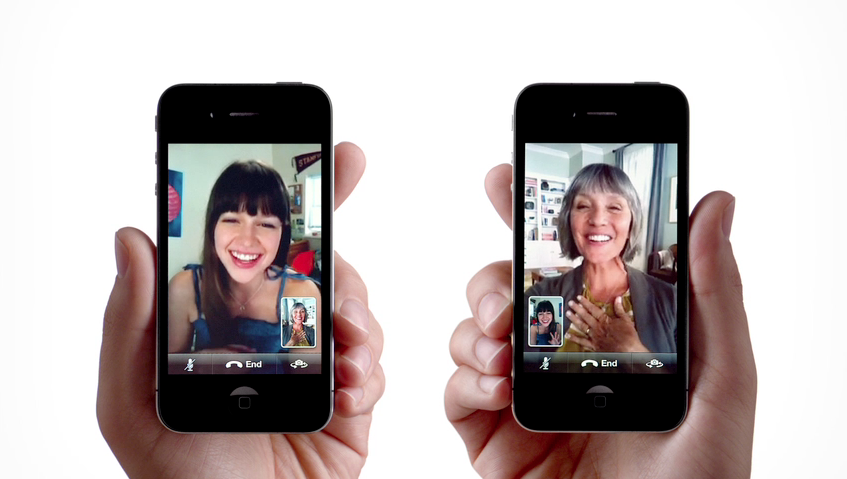
\includegraphics{figures/iphone-face-to-face.png}
	\caption{Still from an Apple advertisement demonstrating the Facetime feature to enable mobile video conferencing.}
	\label{fig:facetime}
\end{marginfigure}

It is not, however, the only way to approach this problem. In their famous paper, \citet{Hollan:1992tz} suggest an alternative approach which they named ``beyond being there''. They argue that seeking to recreate the experience of ``being there'' was in a way an abdication of our responsibility as designers that left an important design space un-explored. In particular, they urge us to think less about ways to minimize the experience of mediation in communication, but to look instead for ways that mediation can add value to interactions. To take this perspective seriously, we need to shift away from a view of face-to-face interaction as being always better than interactions mediated by technology and instead think critically about potential limitations and challenges with face-to-face interaction and potential benefits that mediation can offer. 

Although Hollan and Stornetta focus on creating mediated experiences that rival or surpass face-to-face experiences, I argue that there is another  strategy that deserves our attention. A certain amount of ``being there'' in the form of audio or video is tremendously valuable, as \citet{Ochsman:1974vu} described in their studies. My work focuses on the design of systems that \emph{complement} such experiences by attempting to provide the benefits of mediation in situations where either the users are actually physically co-located, or where they are using a traditional ``being there''-type technology (such as audio or video conferencing).

This equivalence may seem unlikely; why should we accept that systems used in coordination with audio or video conferencing would be similar to those used face-to-face? I will argue that a system that can effectively complement face-to-face interaction when its users could simply set it aside and rely on the (presumed superior) affordances of unfettered verbal communication likely has something to tell us about both design and face-to-face interaction more generally. If these systems can provide value in face-to-face contexts, I will show that they also provide value (perhaps even more value) when used to complement systems that seek to create experiences \emph{like} being face-to-face. Furthermore, true ``distributed'' situations are becoming less common. Heterogenous configurations where some people are co-located and others are remote and alone are becoming more common. In these contexts, a system that doesn't operate effectively between co-located users is unlikely to be broadly useful. Thinking broadly about systems that complement both face-to-face and audio/video sharing will more efficiently lead us to systems effective on both contexts than treating them as separate cases.



% think about listifying this section

% Many of these challenges are common sense, even if they are frequently forgotten when people argue for recreating face-to-face experiences. Face-to-face communication requires relatively explicit turn-taking; multiple speakers in a group make them all largely unintelligible. In mediated environments like chat, simultaneous conversation threads can easily co-exist for long periods of time. There are major identity implications to face-to-face communication. It is difficult to conduct any face-to-face communication without revealing significant information about your identity. In mediated contexts, there are techniques ranging from anonymity to pseudonymity to limit identity disclosing information. Participation in non-mediated interactions is ephemeral, while mediated interaction can easily be archived and represented either in context or after the fact. Participation in face-to-face situations can be limited by confidence, but mediated participation tends to be more disinhibited. \citep{Siegel:1986ve}

% is this a second order effect?
% For a variety of reasons, the power dynamics in social situations are more easily subverted in mediated environments. 

In my work, I focus on a series of ``primary'' contexts: virtual worlds, face-to-face panel discussions, small group seminar discussions, business meetings, remote information sessions, and live-event spectating and describe a system that can complement that ``primary'' experience in a way that enhances the overall experience. Metrics and evaluation strategies vary for each of these pieces, but each project shares a deep interest in trying to fill in the gaps of the ``primary'' interaction space by using the particular strengths of less ``rich'' mediated communication channels. The goal of these interventions is to create environments where people have ways to express themselves non-verbally in addition to whatever existing communication channels exist. By adding mediated communication channels to other existing channels, we can focus on the affordances of each channel to let it do what it does best while addressing the short-comings of each.


% Part of what's attractive about mediated communication systems is that there is a tremendous variety of ways to design and use them once we set aside a desire to recreate face-to-face interaction. Although in this section I've contrasted mediated communication with face-to-face communication in a way that might imply that mediated communication systems are somehow monolithic and self-similar, the survey of related systems in the section to follow will illustrate the tremendous range of potential systems in this space and demonstrate how thoughtful designs can have widely varying impacts on the experience of communication or collaboration. 

% My work takes this general design strategy of adding new communication channels in a few different directions. In this proposal, I will describe my past work looking at meetings in virtual worlds, audience-speaker interaction in presentations, and classroom discussions. I will also lay out my design for a system to support face-to-face meetings with remote participants. These research contexts vary both in the numbers of simultaneous participants, as well as their geographic configuration. Over the course of my work, I have shifted my attention from configurations where all users are remote (\emph{Information Spaces}) to heterogeneous situations where some or all of the participants are co-located (\emph{backchan.nl}, \emph{Tin Can Classroom}, \emph{Tin Can Conference}). 

% TODO Add a paragraph here that preludes some of the design as research ideas (which will be covered in more depth in their own section) as a way of saying that having these themes is part of what makes this research-worthy. 

Across this set of projects, I explore three major research themes:

\begin{description}
	\item[Grounding]{My work uses shared displays in a variety of different capacities. I contend that these kinds of public displays can play a powerful role in helping to ground, in the \citet{Clark:1989uc} sense, a conversation. In particular, shared displays can provide ways to non-verbally acknowledge discourse presentations. By their very shared nature, the contents of shared displays might accelerate the creation of common ground. The different ways that these shared displays operate in my work helps provide insight into both particular design techniques to support grounding as well as the broader discussion around how common ground operates in mediated communication contexts.}
	\item[Non-verbal actions]{As a result of the drive to create a sense of ``being there'', mediated interaction systems failed to consider the ways that we communicate non-verbally, assuming that higher fidelity video and audio would be sufficient to capture that communication. I contend that our non-verbal actions in the physical world are a critical component of body language, and when creating mediated channels we should strive to create new vocabularies of action that enable people to communicate non-verbally. In much the same way that in a shared physical space we can observe people interact with objects around us, so too should people's actions in mediated systems be visible and part of supporting a sense of presence and awareness. How these action vocabularies are constructed and communicated to people is critical to the success of these sorts of systems.}
	\item[Attention]{Adding communication channels forces us to decide how we manage our attention. Which channels do we attend to? How is our attention made visible to others, and how does it affect their impressions of us? Furthermore, how we decide which channels are appropriate for which kind of communication? Although attention is not an inherent design issue, understanding how people think about and enact attention in situations with multiple available communication channels is critical to designing appropriate options and understanding the practices that evolve around them.}
\end{description}

This work will contribute on two levels. First, by creating and deploying interfaces with particular properties, I can provide concrete guidance and insight about particular specific design strategies and interfaces. This is valuable for designers and researchers thinking about how they design this variety of communication systems, a space which based on my interactions with sponsors is increasingly relevant. I will also contribute to the broader discourse about the three research themes laid out above. In each case there are both broader theoretical contributions to be made as well as specific findings that contribute to scholarly discussions about these issues.




% I have focused my work in a number of ways. Although many of the interfaces proposed as being ``beyond being there'' in their original paper are asynchronous systems, I focus exclusively on synchronous experiences -- co-temporal experiences where participants are communicating and using a system at the same time. I focus primarily on medium sized groups and crowds. Although the groups are always interacting co-temporally, they are sometimes all in one physical place, and sometimes geographically distributed. 

% It can be difficult to describe exactly what the contributions of design focused research can be. In my work, I see two major categories of contributions. First, by building systems and testing them \emph{in situ} I can provide concrete guidance about particular specific design strategies and interfaces were used by users in practice. This is valuable for designers and researchers thinking about how they design non-verbal communication systems in their own work. I also engage with broader theoretical questions about attention, signaling, grounding. By contributing to these larger discourses with specific findings in studies of my own systems, I hope to contribute to broader discussions in computer mediated communication. 

% gotta really settle on what my themes are going to be here. current list is:
%  - attention (solid)
%  - signaling (erm - what is this exactly?)
%  - grounding (I like)
%  - 


% It can be difficult to describe exactly what the contributions of design focused research can be. Is making something that people describe as useful a sufficient outcome, or should we expect more? I conceive of my research as being a kind of design cartographer. Given the design space I outlined earlier, I try to identify and describe compelling and effective design strategies. Beyond the specific contributions of design elements that are valuable, I step back from the specifics of each system and theorize about general themes that are relevant to any sort of design work in the space. In this case, these are themes like stages, performative attention and contribution, norms, power dynamics, and grounding. By contributing in both of these ways, I seek to support designers and researchers working both with modern constraints as well as contribute theoretically to ways of thinking about design of co-temporal mediated experiences that will give us the tools to think about as-yet-unimagined design spaces.

% At that scale, I find that the benefits of being face-to-face are strongest and successful interventions are quite difficult to produce. (Leave the research strategic points for later?)

% talk about general themes + backchannels

In this proposal, I will start with a survey of relevant related systems, as well as briefly touching on experimental, theoretical, and methodological work that plays a significant role in my work. Then I will describe the arc of my  work with a focus on my final project: Tin Can. Finally, I will describe in general terms the contributions and potential impact of this work.


\section{Design Research/Methodology}

I want to talk about this as an overall strategy, but not sure where exactly to put it. It doesn't really fit in the stages discussion (which will occupy most of chapter 2? or chapter 3?). Really, I think I need to take a step back on the intro and split it up a little more rigorously. Section ideas:

 * Being There
 * Complementing, Not Replacing
 * Domains and Themes
 * Design as Research
 * Intro to Rest
